%%%%%%%%%%%%%%%%%%%%%%%%%%%%%%%%%%%%%%%%%%%%%%%%%%%%%%%%%%
\frame {\frametitle{The CAP Theorem}
%%%%%%%%%%%%%%%%%%%%%%%%%%%%%%%%%%%%%%%%%%%%%%%%%%%%%%%%%%
\begin{itemize}
	\item {\bf Frequently cited distributed systems theorem}

	\vspace{20pt}

	\item {\bf Relates the following three properties}
	\begin{itemize}
		\item C: Consistency
		\begin{itemize}
			\item One-copy semantics, linearizability, atomicity, total order
			\item Every operation must appear to take effect in a single indivisible point in time between its invocation and response
		\end{itemize}
		\item A: Availability
		\begin{itemize}
			\item Every client's request is served (receives a response) unless a
client fails (despite a strict subset of server nodes failing) 
		\end{itemize}
		\item P: Partition tolerance
		\begin{itemize}
			\item A system functions properly even if the network is allowed to lose arbitrarily many messages sent from one node to another
		\end{itemize}
	\end{itemize}

\end{itemize}
}

%%%%%%%%%%%%%%%%%%%%%%%%%%%%%%%%%%%%%%%%%%%%%%%%%%%%%%%%%%
\frame {\frametitle{The CAP Theorem}
%%%%%%%%%%%%%%%%%%%%%%%%%%%%%%%%%%%%%%%%%%%%%%%%%%%%%%%%%%
\begin{itemize}
	\item {\bf In the folklore interpretation, the theorem says:}
	\item[] C, A, P: pick two
\end{itemize}

\begin{figure}[h]
	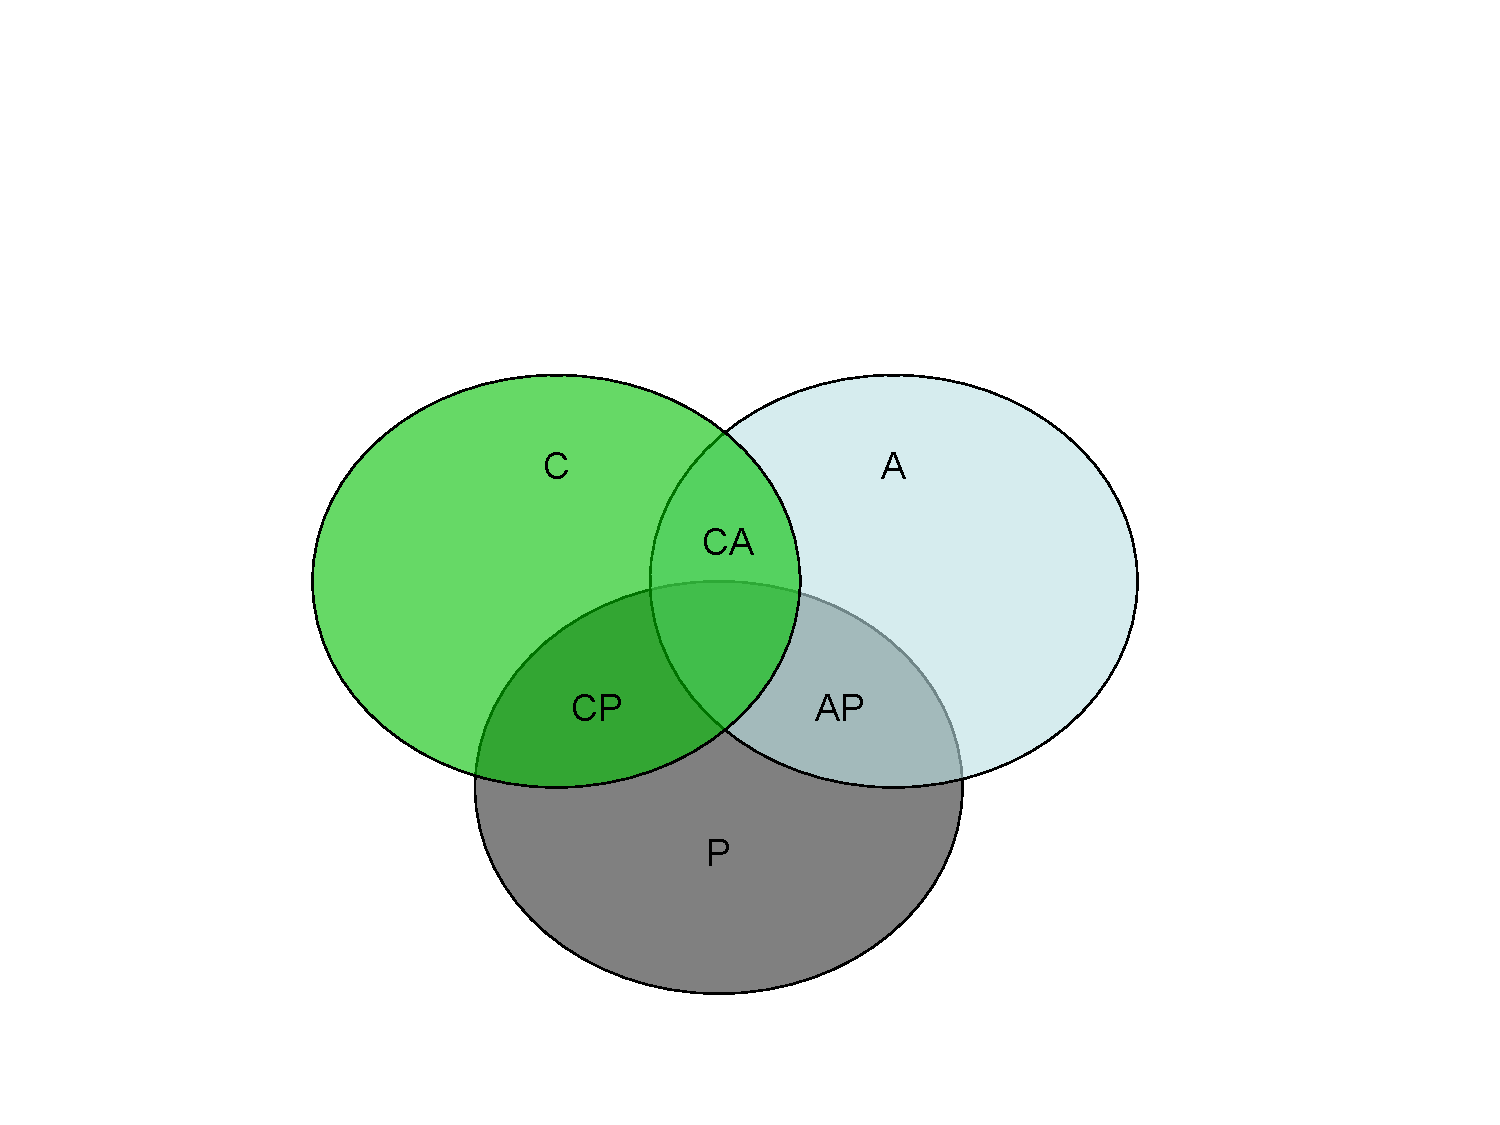
\includegraphics[scale=0.3]{./figures/cap_pick2}
\end{figure}
}

%%%%%%%%%%%%%%%%%%%%%%%%%%%%%%%%%%%%%%%%%%%%%%%%%%%%%%%%%%
\frame {\frametitle{Precautions: be careful with CA}
%%%%%%%%%%%%%%%%%%%%%%%%%%%%%%%%%%%%%%%%%%%%%%%%%%%%%%%%%%
\begin{itemize}
	\item {\bf Sacrificing P (partition tolerance)}

	\vspace{20pt}

	\item {\bf Negating:} A system functions properly even if the network is allowed to lose arbitrarily many messages sent from one node to another 

	\vspace{20pt}

	\item {\bf Yields:} A system {\color{red}does not} function properly even if the network is allowed to lose arbitrarily many messages sent from one node to another
	\begin{itemize}
		\item This implies sacrificing C or A, \textit{i.e.,} the system does not work
	\end{itemize}
\end{itemize}
}

%%%%%%%%%%%%%%%%%%%%%%%%%%%%%%%%%%%%%%%%%%%%%%%%%%%%%%%%%%
\frame {\frametitle{Precautions: be careful with CA}
%%%%%%%%%%%%%%%%%%%%%%%%%%%%%%%%%%%%%%%%%%%%%%%%%%%%%%%%%%
\begin{itemize}
	\item {\bf Negating P:} A system function properly if the network is {\color{red}not allowed} to lose arbitrarily many messages

	\vspace{20pt}

	\item {\bf However, in practice:} It is not possible to choose whether the network will lose messages! This either happens or not

	\vspace{20pt}

	\item {\bf One can argue that not ``arbitrarily'' many messages will be lost}
	\begin{itemize}
		\item But ``a lot'' of them might be (before the network repairs)
		\item In the meantime, either C or A is sacrificed
	\end{itemize}
\end{itemize}
}

%%%%%%%%%%%%%%%%%%%%%%%%%%%%%%%%%%%%%%%%%%%%%%%%%%%%%%%%%%
\frame {\frametitle{CAP in practice}
%%%%%%%%%%%%%%%%%%%%%%%%%%%%%%%%%%%%%%%%%%%%%%%%%%%%%%%%%%
\begin{itemize}
	\item {\bf In practical distributed systems:}
	\begin{itemize}
		\item Partitions may occur
		\item This is not under your control, as a system designer
	\end{itemize}

	\vspace{20pt}

	\item {\bf Designer's choice:}
	\begin{itemize}
		\item {\color{red}You choose} whether you want your system in C or A, when/if (temporary) partitions occur
	\end{itemize}

	\vspace{20pt}

	\item {\bf In summary:}
	\begin{itemize}
		\item CAP is a fundamental theorem stating the tradeoffs among different system properties
		\item {\color{red}Practical distributed systems are either in CP or AP}
		\item {\bf The choice (C vs. A) depends on your application logic}
	\end{itemize}
\end{itemize}
}

%%%%%%%%%%%%%%%%%%%%%%%%%%%%%%%%%%%%%%%%%%%%%%%%%%%%%%%%%%
\frame {\frametitle{CAP in theory}
%%%%%%%%%%%%%%%%%%%%%%%%%%%%%%%%%%%%%%%%%%%%%%%%%%%%%%%%%%
\begin{itemize}
	\item {\bf Historical notes:}
	\begin{itemize}
		\item First stated by Eric Brewer at the PODC 2000 keynote
		\item Formally proved by Gilbert and Lynch, 2002
	\end{itemize}

	\vspace{20pt}

	\item {\bf GL Theorems:}
	\begin{itemize}
		\item Asynchronous / partially synchronous network models
		\item Read/Write data objects
		\item Finer definitions of Availability and Consistency
	\end{itemize}

	\vspace{20pt}

	\item {\bf Further readings:}
	\begin{itemize}
		\item (Fischer, Lynch and Patterson) FLP impossibility result
		\item t-connected CAP
	\end{itemize}
\end{itemize}
}

%%%%%%%%%%%%%%%%%%%%%%%%%%%%%%%%%%%%%%%%%%%%%%%%%%%%%%%%%%
\frame {\frametitle{CAP: some illustrative choices}
%%%%%%%%%%%%%%%%%%%%%%%%%%%%%%%%%%%%%%%%%%%%%%%%%%%%%%%%%%
\begin{itemize}
	\item {\bf CP:}
	\begin{itemize}
		\item BigTable (Google), HBase, ...
		\item Coordination systems: ZooKeeper, etcd, ...
	\end{itemize}

	\vspace{40pt}

	\item {\bf AP:}
	\begin{itemize}
		\item Amazon Dynamo, CouchDB, Cassandra, SimpleDB, Riak, Voldemort (LinkedIn), ...
	\end{itemize}
\end{itemize}
}
